\documentclass[conference]{IEEEtran}
\IEEEoverridecommandlockouts
\usepackage{cite}
\usepackage{amsmath,amssymb}
\usepackage{graphicx}
\usepackage{booktabs}
\usepackage{array}
\usepackage{url}
\usepackage[T1]{fontenc}
\usepackage{textcomp}
\usepackage{xcolor}
\usepackage{tikz}
\usetikzlibrary{arrows.meta,positioning,fit,shapes.geometric}
\usepackage[colorlinks=true,allcolors=blue!50!black]{hyperref}
\def\BibTeX{{\rm B\kern-.05em{\sc i\kern-.025em b}\kern-.08em T\kern-.1667em\lower.7ex\hbox{E}\kern-.125em X}}

\begin{document}

\title{Does Cross-Attention Fusion of ECG and Pulse Signals Verify ICU Arrhythmia Alarms? A Leakage-Audited Study on PhysioNet/CinC 2015 and VTaC}

\author{\IEEEauthorblockN{Veerbhadra Mahant, Ved Jadhav, Sharvil Patil, and Roshani Raut}
\IEEEauthorblockA{Pimpri Chinchwad College of Engineering, Pune\\
Pune, India\\
veerbhadra.mahant24@pccoepune.org, ved.jadhav24@pccoepune.org,\\
sharvil.patil24@pccoepune.org}}

\maketitle

\begin{abstract}
Intensive-care monitors raise many false arrhythmia alarms, and alarm fatigue can delay the response to true ones. We ask whether a second, independent pulse signal (photoplethysmogram, PPG) can verify an ECG-triggered alarm, and whether cross-attention fusion is the right way to combine the two. We compared 14 neural architectures, six classical algorithms on 266 engineered features, a hybrid attention CNN-GRU recipe and ensembles on two open datasets, PhysioNet/CinC Challenge 2015 (592-record PPG cohort) and VTaC (4,542 ventricular tachycardia alarms), using a leakage-free protocol with inner validation sets, 10 seeds and corrected statistics. Removing a validation leak from our first code version lowered the F1 of the proposed cross-attention model from 0.774 to 0.699 and erased its advantage over concatenation ($\Delta$F1 $=+0.006$, 95\% CI $-0.015$ to $+0.028$). Classifiers on engineered features (F1 up to 0.818) and a hybrid deep recipe (F1 0.828 on Challenge 2015; F1 0.858 and AUC 0.966 on VTaC) clearly beat plain cross-attention. Counterfactual tests show that the fused models ignore ECG-to-pulse timing: substituting another patient's same-label PPG changes AUC by less than 0.03, and attention does not track measured pulse transit time ($\rho=-0.04$). Transfer between datasets is asymmetric: models trained on Challenge 2015 reach an F1 of only 0.56 to 0.60 on VTaC when the ECG is used. The pulse works as a patient-agnostic evidence cue, not as a timing check; training and feature engineering matter more than the fusion layer; and single-dataset results overstate generalization. This is a research prototype without prospective validation.
\end{abstract}

\begin{IEEEkeywords}
false alarm reduction, intensive care unit, arrhythmia alarm verification, multimodal fusion, cross-attention, electrocardiogram, photoplethysmogram, data leakage, pulse transit time, PhysioNet
\end{IEEEkeywords}

%=====================================================================
\section{Introduction}
Bedside monitors in intensive care units (ICUs) generate many arrhythmia alarms, and a large share of them are false. An observational study of consecutive ICU patients and a review of the alarm-fatigue literature both report that this burden desensitizes staff and can slow the response to true alarms \cite{drew2014alarm,cvach2012alarm}. Ventricular tachycardia (VT) alarms are among the most frequent life-threatening alarms, and false VT alarms have proved the hardest to suppress reliably \cite{lehman2023vtac,clifford2016false}. Most monitors raise an alarm from the electrocardiogram (ECG) alone. Electrode motion or muscle noise corrupts the ECG, so it also corrupts the signal that would be used to check the alarm.

A second, physically independent signal can help. The photoplethysmogram (PPG) and the arterial blood pressure (ABP) waveform show whether an electrical event was followed by a mechanical pulse, and they fail under different conditions than the ECG. A genuine arrhythmia should disturb both signals, while an ECG artifact should leave the pulse intact. Earlier work used this idea with hand-crafted ABP features \cite{aboukhalil2008abp}, in the 2015 PhysioNet/Computing in Cardiology Challenge \cite{clifford2015challenge,clifford2016false}, and with deep models. The closest deep models are the attention-based convolutional and recurrent networks of Mousavi et al. \cite{mousavi2020attention}, which reported a sensitivity of 93.88\% and a specificity of 92.05\% with three signals, and the contrastive approach of Zhou et al. \cite{zhou2022contrastive}, which adds learned alarm-type embeddings.

We started from a specific hypothesis. A transformer-style \emph{cross-attention} layer \cite{vaswani2017attention}, in which ECG features query PPG features, should learn the pulse transit time (PTT) between the electrical beat and the arriving pulse, and this comparison should verify alarms better than a model that sees one signal or simply concatenates both. The research problem has two parts: (i) does fusing ECG and pulse improve alarm verification, and (ii) if it does, does the attention-based alignment explain the gain? Our first code version answered (ii) positively (F1 of 0.774 for cross-attention), but that estimate was biased upward because the best epoch was selected on the same fold that was reported. This paper starts from a re-run under a leakage-free protocol.

Our objectives are to (1) compare cross-attention with ECG-only, PPG-only and concatenation baselines at matched parameter count; (2) benchmark it against stronger classical, deep, hybrid and ensemble alternatives on two datasets; (3) test with counterfactual perturbations whether fusion models use ECG-to-pulse timing; (4) measure robustness to noise and sensor loss, and transfer across datasets; and (5) report every result with corrected statistics, including those that contradict the original hypothesis.

Section~\ref{sec:methods} describes the datasets, preprocessing, models, training, implementation and mathematics. Section~\ref{sec:results} gives the results, a discussion and the limitations. Section~\ref{sec:conclusion} concludes.

%=====================================================================
\section{Methods}\label{sec:methods}

\subsection{Overview}
Fig.~\ref{fig:pipeline} summarizes the pipeline. Each alarm event is represented by a 10~s window of ECG and a pulse channel that ends exactly at the alarm onset. Three families of models are trained on the same windows and splits: neural networks on the raw signals, classical learners on engineered features, and a hybrid deep recipe; their predictions are combined in ensembles.

\begin{figure*}[t]
\centering
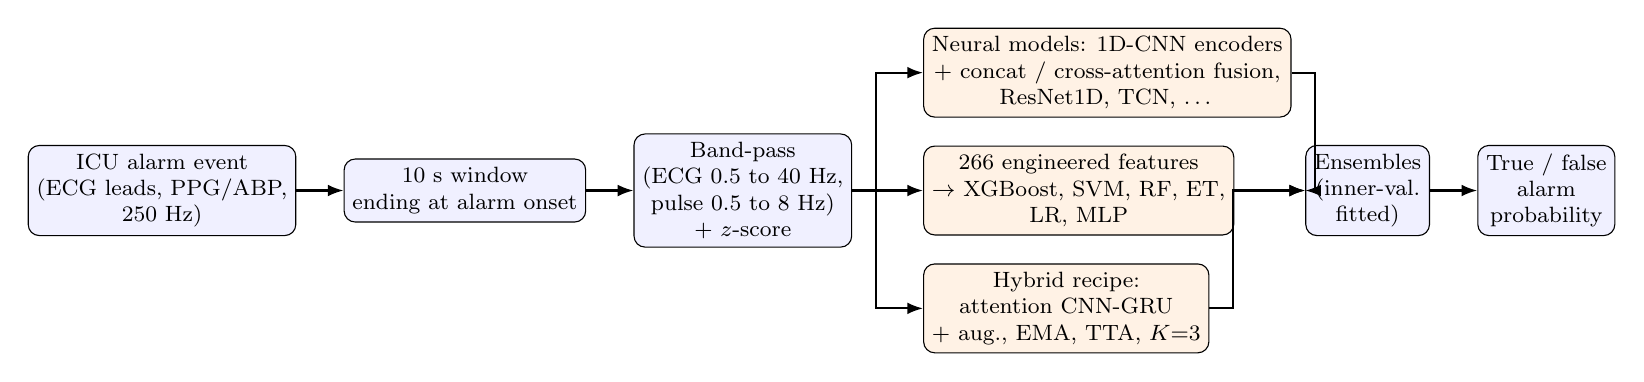
\begin{tikzpicture}[font=\footnotesize, node distance=5mm and 6mm,
  box/.style={draw, rounded corners, align=center, minimum height=8mm, inner sep=3pt, fill=blue!6},
  big/.style={draw, rounded corners, align=center, minimum height=8mm, inner sep=3pt, fill=orange!10},
  arr/.style={-{Latex[length=2mm]}, thick}]
\node[box] (raw) {ICU alarm event\\(ECG leads, PPG/ABP,\\250~Hz)};
\node[box, right=of raw] (win) {10~s window\\ending at alarm onset};
\node[box, right=of win] (pre) {Band-pass\\(ECG 0.5 to 40~Hz,\\pulse 0.5 to 8~Hz)\\+ $z$-score};
\node[big, above right=2mm and 9mm of pre] (nn) {Neural models: 1D-CNN encoders\\+ concat / cross-attention fusion,\\ResNet1D, TCN, \dots};
\node[big, right=9mm of pre] (cl) {266 engineered features\\$\to$ XGBoost, SVM, RF, ET,\\LR, MLP};
\node[big, below right=2mm and 9mm of pre] (hy) {Hybrid recipe:\\attention CNN-GRU\\+ aug., EMA, TTA, $K{=}3$};
\node[box, right=9mm of cl] (ens) {Ensembles\\(inner-val.\\fitted)};
\node[box, right=of ens] (out) {True / false\\alarm\\probability};
\draw[arr] (raw)--(win); \draw[arr] (win)--(pre);
\draw[arr] (pre.east)--++(3mm,0)|-(nn.west);
\draw[arr] (pre.east)--(cl.west);
\draw[arr] (pre.east)--++(3mm,0)|-(hy.west);
\draw[arr] (nn.east)--++(3mm,0)|-(ens.west);
\draw[arr] (cl.east)--(ens.west);
\draw[arr] (hy.east)--++(3mm,0)|-(ens.west);
\draw[arr] (ens)--(out);
\end{tikzpicture}
\caption{Overview of the verification pipeline. All stages see only samples up to the alarm onset; hyper-parameters, thresholds and ensemble weights are fitted on inner validation records of each training fold.}
\label{fig:pipeline}
\end{figure*}

\subsection{Data collection}
No new recordings were collected; all data are public, de-identified and were obtained from their original hosts. Table~\ref{tab:datasets} lists every dataset with its citation and source URL. Cohort statistics below come from the audit files written by our preprocessing scripts.

\begin{table*}[t]
\caption{Datasets used in this study, with required citations and source URLs.}
\label{tab:datasets}
\centering
\small
\begin{tabular}{p{2.6cm}p{3.7cm}p{3.7cm}p{6.3cm}}
\toprule
\textbf{Dataset} & \textbf{Role} & \textbf{Content used} & \textbf{Citation and source URL}\\
\midrule
PhysioNet/CinC Challenge 2015 training set & Primary training and cross-validation & 750 ICU records, 5 alarm types, expert true/false label; 592-record PPG cohort, 724-record recovered cohort & \cite{clifford2015challenge,clifford2015cincdata}; \url{https://physionet.org/content/challenge-2015/1.0.0/}\\
VTaC v1.1 & Second training/test set, official patient-disjoint split & 5,037 annotated VT alarms (3 US hospitals, 3 monitor vendors); 4,542 used & \cite{lehman2023vtac,lehman2024vtacdata}; \url{https://physionet.org/content/vtac/}\\
MIMIC PERform AF & External AF-screening task (35 subjects) & 19 AF, 16 non-AF subjects; ECG + PPG at 125~Hz & \cite{charlton2025perform,charlton2022beats}; \url{https://zenodo.org/records/15906524}\\
MIT-BIH Noise Stress Test & Synthetic noise injection (robustness) & Baseline wander, electrode motion, muscle artifact & \cite{moody1984nstdb}; \url{https://physionet.org/content/nstdb/1.0.0/}\\
MIT-BIH Arrhythmia Database & Validation of the R-peak detector & 10 records & \cite{moody2001mitbih}; \url{https://physionet.org/content/mitdb/1.0.0/}\\
PaPaGei pretrained weights & Foundation-model comparison (not a dataset) & PPG encoders PaPaGei-S/-P & \cite{pillai2025papagei}; \url{https://zenodo.org/records/13983110}\\
\bottomrule
\end{tabular}
\end{table*}

\emph{Challenge 2015.} The training set contains 750 five-minute ICU records at 250~Hz; the alarm is raised at the 300~s mark, and every alarm carries an expert true or false label for one of five types (asystole, extreme bradycardia, extreme tachycardia, ventricular tachycardia, ventricular flutter/fibrillation) \cite{clifford2015challenge,clifford2016false}. The 500-record test set was never released, so record-wise cross-validation is the appropriate evaluation. Of the 750 records, 627 carry PPG, 343 carry ABP and all have a second ECG lead. The original \emph{PPG cohort} has 592 records (37.7\% true alarms). A \emph{recovered cohort} of 724 records (39.6\% true) substitutes ABP for the pulse where PPG is absent (132 records) and excludes 26 records whose window is too short or nearly flat-lined.

\emph{VTaC.} VTaC contains 5,037 annotated VT alarm events with at least two independent expert annotators each \cite{lehman2023vtac}; v1.1 additionally releases per-annotator votes. The host throttles each connection, so we downloaded only the window $[-60~\mathrm{s},+30~\mathrm{s}]$ around each alarm onset using parallel HTTP range requests (about 1~GB instead of 18~GB). After excluding 292 events without a pulse channel and 203 low-quality windows, 4,542 events from 2,138 patients remain (28.0\% true alarms); the official patient-disjoint split yields 3,662 training, 453 validation and 427 test events. Hospital and device identifiers are not released.

\emph{Auxiliary data.} MIMIC PERform AF (35 subjects, 125~Hz) is used only for an AF-screening task, with 60 evenly spaced 10~s windows per subject (2,100 windows) \cite{charlton2025perform,charlton2022beats}. The MIT-BIH Noise Stress Test supplies real noise for stress testing \cite{moody1984nstdb}.

\subsection{Data preparation}
\emph{Windowing.} The headline task window is the 10~s that end exactly at the alarm onset; no post-alarm samples enter any model input. The 30~s after the onset are read only by a separate time-to-verdict analysis. This decision-time alignment replaced an earlier center-aligned window.

\emph{Preprocessing.} Signals are resampled to 250~Hz and filtered with a zero-phase fourth-order Butterworth band-pass (ECG 0.5 to 40~Hz; pulse 0.5 to 8~Hz), then $z$-normalized per window, so that nothing is fitted across windows and no train/test statistics leak. A simple per-channel quality score (flat-line variance and clipping fraction) removes windows below a quality threshold of 0.05.

\emph{Splits.} Challenge 2015 uses record-wise 5-fold cross-validation repeated for 10 seeds (the seed changes the fold assignment). VTaC uses the official patient-disjoint split with 5 to 10 seeds. Inside every training fold, 15\% of the records form an \emph{inner validation set} that drives early stopping, model selection, calibration, thresholds and ensemble weights; the outer test fold is evaluated once. All models see identical splits, so comparisons are paired.

\subsection{Model selection}
\emph{Parameter-matched baseline ladder.} The core comparison uses four variants matched to about 261k parameters (single-signal models are widened): ECG-only, PPG-only, concatenation fusion, and the proposed cross-attention fusion. Each signal passes through its own (not weight-shared) 1D-CNN encoder (channels 32/64/128, kernel sizes 15/9/7, pooling 2, dropout 0.3) that outputs a feature \emph{sequence}. In cross-attention (4 heads, dimension 128, positional encodings) the ECG sequence supplies the queries and the PPG sequence the keys and values; a shallow head (64 hidden units) produces the alarm logit.

\emph{Rivals.} We added four fusion variants (bidirectional cross-attention, joint transformer with modality embeddings, bottleneck-token fusion, quality-gated cross-attention) and a baseline zoo on a 2-channel early-fusion input: ResNet1D \cite{he2016resnet}, InceptionTime \cite{fawaz2020inceptiontime}, a bidirectional GRU, a TCN \cite{bai2018tcn}, a patch transformer and a compact diagonal state-space model. In total 14 neural architectures were compared.

\emph{Classical models.} 266 engineered features (HRV, ECG morphology proxies, wavelet and spectral features, PPG pulse features, ECG-PPG agreement such as PTT statistics and beat-count ratios in the last 5~s, and signal-quality indices) feed six algorithms: logistic regression, RBF-SVM, random forest, extra trees, XGBoost \cite{chen2016xgboost} and an MLP. ECG beats are detected with a Pan-Tompkins-style detector \cite{pantompkins1985}. Thirty random hyper-parameter configurations per fold and algorithm are scored on the inner validation set only. A first, 53-feature gradient-boosting baseline (``features v1'') is also reported.

\emph{Hybrid deep recipe.} Following the attention CNN-RNN design of \cite{mousavi2020attention} (our re-implementation from the published description, not the authors' code), a 48-configuration grid (6 architectures $\times$ augmentation $\times$ loss $\times$ learning rate) was declared in advance and scored by inner-validation AUC. The winner, an attention CNN-GRU with augmentation, focal loss and learning rate $10^{-3}$, was combined with AdamW \cite{loshchilov2019adamw}, a one-cycle schedule \cite{smith2019onecycle}, weight EMA, test-time augmentation and a 3-member ensemble. Hybrid variants that append the 53 agreement features to the deep representation were also tested.

\emph{Ensembles.} Logit mean, probability mean, a logistic-regression stacker and greedy selection are all fitted on inner-validation predictions only.

\emph{Self-supervised pretraining and foundation models.} Contrastive, masked-reconstruction and cross-modal-prediction objectives were pretrained on VTaC pre-alarm segments of training/validation patients only. The PaPaGei PPG foundation model \cite{pillai2025papagei} was evaluated frozen (linear probe), as a frozen encoder inside fusion models, and with last-block fine-tuning. ECG-FM \cite{mckeen2024ecgfm} weights were downloaded but not run, because the model needs a 12-lead 500~Hz input and a compiler toolchain that was unavailable.

\subsection{Training procedure}
Baseline-ladder models use Adam with learning rate $10^{-3}$, weight decay $10^{-4}$, batch size 16, at most 60 epochs and early stopping (patience 10) on inner-validation F1, with focal loss. The hybrid recipe uses AdamW (weight decay $10^{-2}$), a one-cycle schedule with 15\% warm-up, gradient clipping at 1.0, batch 32 (64 on VTaC), at most 30 epochs (20 on VTaC) and early stopping on inner-validation AUC. Augmentation (training only) comprises a joint circular time shift of $\pm1$~s, per-channel amplitude scaling, additive Gaussian noise and a random 1~s dropout of one modality. Hyper-parameters of the ladder are fixed in a configuration file and not tuned per variant. Class imbalance is handled by class weighting or focal loss, not resampling.

\subsection{Implementation details and tools}
Code is written in Python with PyTorch \cite{paszke2019pytorch}, scikit-learn \cite{pedregosa2011sklearn}, XGBoost \cite{chen2016xgboost}, SciPy, PyWavelets, pandas and the WFDB package for reading PhysioNet records \cite{goldberger2000physionet}. Experiments ran on a single workstation GPU (RTX PRO 4000 Blackwell, 24~GB) with 20 CPU cores; neural folds train in seconds to minutes. The repository holds the code, configurations and the result files from which every table and figure here was produced.

\subsection{Mathematical formulation}
Let $E,P\in\mathbb{R}^{T'\times d}$ be the ECG and PPG feature sequences (with positional encodings added). Cross-attention computes
\begin{equation}
\mathrm{Attn}(E,P)=\mathrm{softmax}\!\left(\frac{(EW_Q)(PW_K)^{\top}}{\sqrt{d_k}}\right)PW_V,
\label{eq:attn}
\end{equation}
so each ECG time step aggregates the PPG steps judged relevant. Concatenation fusion instead stacks the pooled features. Training uses the focal loss \cite{lin2017focal}
\begin{equation}
\mathcal{L}=-\alpha_t(1-p_t)^{\gamma}\log p_t,\quad \gamma=2,
\label{eq:focal}
\end{equation}
where $p_t$ is the predicted probability of the true class. The pulse transit time of beat $i$ is $\mathrm{PTT}_i=t^{\mathrm{foot}}_i-t^{R}_i$ (R-peak to PPG foot). Classification is scored by F1 $=2\,\mathrm{TP}/(2\,\mathrm{TP}+\mathrm{FP}+\mathrm{FN})$, AUC, and the Challenge 2015 score
\begin{equation}
S=\frac{\mathrm{TP}+\mathrm{TN}}{\mathrm{TP}+\mathrm{TN}+\mathrm{FP}+5\,\mathrm{FN}},
\label{eq:score}
\end{equation}
in which a missed true alarm costs five false alarms \cite{clifford2015challenge}. For two models evaluated on $J$ paired folds, the Nadeau-Bengio corrected resampled $t$-statistic \cite{nadeau2003inference} is
\begin{equation}
t=\frac{\bar d}{\sqrt{\left(\frac{1}{J}+\frac{n_{\mathrm{test}}}{n_{\mathrm{train}}}\right)s_d^{2}}},
\label{eq:nb}
\end{equation}
with $\bar d$ and $s_d^2$ the mean and variance of the paired F1 differences. We additionally use a paired record-level bootstrap with 5,000 resamples \cite{efron1994bootstrap}, in which the same resample is applied to both models, and Holm correction \cite{holm1979} over a comparison family fixed in the configuration file before the final runs. A finding is called robust only if both tests agree after correction. The safety layer applies temperature scaling \cite{guo2017calibration} and certifies a suppression threshold with an exact Clopper-Pearson upper bound on the miss rate \cite{clopper1934}. The repository also contains a TRIPOD+AI reporting checklist \cite{collins2024tripod}.

%=====================================================================
\section{Results and Discussion}\label{sec:results}

\subsection{Effect of removing the validation leak}
The original training script selected the best epoch and stopped training on the same fold it then reported. With a separate inner validation set and 10 seeds, every score fell (Fig.~\ref{fig:leak}): the cross-attention F1 dropped from 0.774 to 0.699 and its advantage over concatenation shrank from $+0.024$ to $+0.006$ (bootstrap 95\% CI $-0.015$ to $+0.028$). The leak came from our earlier code, not from the method. We archived the original numbers and use them nowhere else.

\begin{figure}[t]
\centering
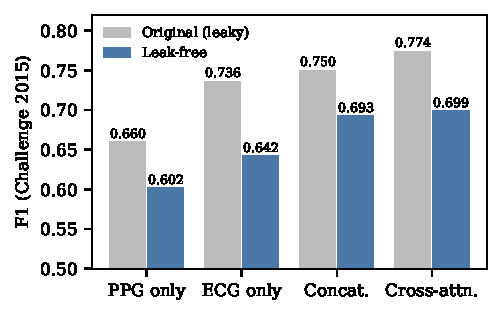
\includegraphics[width=\columnwidth]{figures/leakage.pdf}
\caption{F1 on Challenge 2015 before and after removing the validation leak.}
\label{fig:leak}
\end{figure}

\subsection{Leaderboards}
Tables~\ref{tab:cinc} and~\ref{tab:vtac} and Fig.~\ref{fig:leaderboard} give the main comparison (threshold 0.5; means over seeds and folds).

\begin{table}[t]
\caption{Challenge 2015, PPG cohort (592 records), 5-fold CV $\times$ 10 seeds.}
\label{tab:cinc}
\centering
\small
\begin{tabular}{lccc}
\toprule
Model & Acc. & F1 & AUC\\
\midrule
Ensemble, 10 models (logit mean) & 0.876 & 0.827 & 0.948\\
XGBoost, features v2 & 0.871 & 0.818 & 0.939\\
Extra Trees, features v2 & 0.867 & 0.802 & 0.947\\
Random Forest, features v2 & 0.863 & 0.795 & 0.938\\
MLP, features v2 & 0.857 & 0.802 & 0.927\\
SVM (RBF), features v2 & 0.852 & 0.791 & 0.928\\
Logistic reg., features v2 & 0.852 & 0.801 & 0.928\\
HistGB, features v1 & 0.851 & 0.798 & 0.918\\
ResNet1D & 0.820 & 0.760 & 0.884\\
TCN & 0.810 & 0.751 & 0.887\\
InceptionTime & 0.796 & 0.732 & 0.876\\
CNN cross-attention (proposed) & 0.765 & 0.699 & 0.841\\
CNN concatenation & 0.757 & 0.693 & 0.836\\
\midrule
Hybrid deep recipe (10 seeds) & 0.871 & 0.828 & 0.932\\
Ensemble incl. hybrid (5 seeds) & 0.878 & 0.830 & 0.950\\
\bottomrule
\end{tabular}
\end{table}

\begin{table}[t]
\caption{VTaC, official split (427 test events), 5 seeds.}
\label{tab:vtac}
\centering
\small
\begin{tabular}{lccc}
\toprule
Model & Acc. & F1 & AUC\\
\midrule
Hybrid deep recipe & 0.913 & 0.858 & 0.966\\
Ensemble incl. hybrid (logit mean) & 0.912 & 0.844 & 0.957\\
Ensemble, 10 models (logit mean) & 0.910 & 0.839 & 0.955\\
MLP, features v2 & 0.900 & 0.821 & 0.949\\
XGBoost, features v2 & 0.895 & 0.814 & 0.942\\
SVM (RBF), features v2 & 0.891 & 0.806 & 0.948\\
CNN bidirectional cross-attention & 0.857 & 0.775 & 0.933\\
TCN & 0.856 & 0.760 & 0.919\\
ResNet1D & 0.852 & 0.750 & 0.915\\
CNN cross-attention (proposed) & 0.844 & 0.746 & 0.915\\
CNN concatenation & 0.837 & 0.744 & 0.909\\
\bottomrule
\end{tabular}
\end{table}

\begin{figure*}[t]
\centering
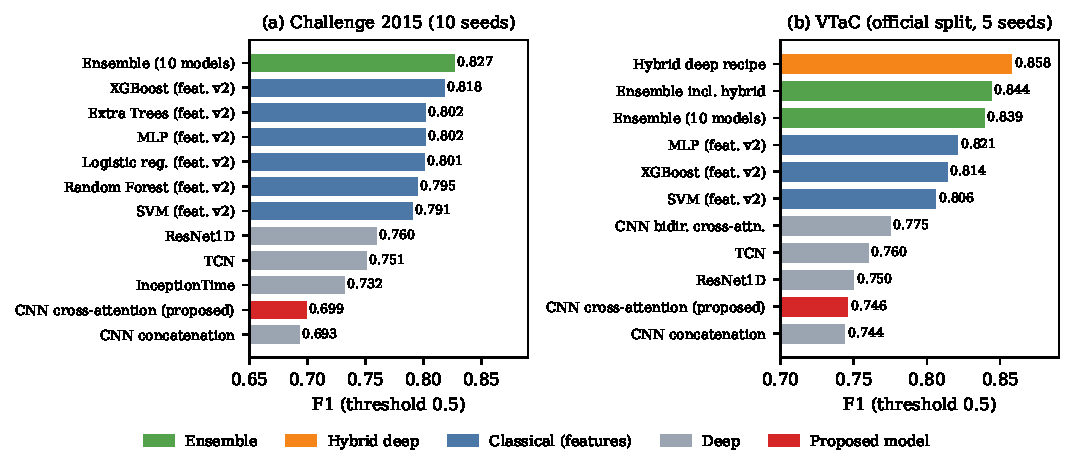
\includegraphics[width=0.92\textwidth]{figures/leaderboard.pdf}
\caption{F1 leaderboards (threshold 0.5). The originally proposed cross-attention model (red) ranks near the bottom on both datasets.}
\label{fig:leaderboard}
\end{figure*}

On Challenge 2015 the proposed cross-attention network ranks 12th of the 13 models in Table~\ref{tab:cinc} by F1, behind every classical model on engineered features and behind ResNet1D, TCN and InceptionTime. The best leak-free results come from the 10-model ensemble (accuracy 0.876) and from the hybrid deep recipe (F1 0.828, AUC 0.932). The ensemble's F1 advantage over the best classical model is within noise ($+0.008$, CI $-0.007$ to $+0.022$), but its advantage over cross-attention is $+0.128$ (CI $+0.094$ to $+0.161$). On VTaC the hybrid recipe leads (F1 0.858, AUC 0.966); differences among the top three models are inside bootstrap noise, whereas the gap to cross-attention is $+0.11$ F1 (CI $+0.07$ to $+0.15$). Fusion does help on VTaC: ECG-only reaches F1 0.709 and PPG-only 0.566, against 0.744 for concatenation.

\emph{Caveat on the hybrid recipe.} Its configuration was selected on inner-validation scores of Challenge 2015 folds. Those records are test records in other seeds and folds, so a small optimistic bias is possible. The same recipe was applied to VTaC without re-tuning, and a shuffled-label control gave a chance-level AUC of 0.57, so we found no evidence of leakage. A recipe ablation (Table~\ref{tab:ablation}) shows that the largest single post-training ingredient is weight averaging (EMA), and part of the gap to the baseline CNNs is a trainer effect (optimizer, regularization, ensembling) rather than an architecture effect, because the baselines use a different trainer.

\begin{table}[t]
\caption{Ablation of the hybrid recipe, Challenge 2015 (10 seeds, paired against the full recipe; SE over seeds).}
\label{tab:ablation}
\centering
\small
\begin{tabular}{lccc}
\toprule
Variant & F1 & AUC & $\Delta$F1 (SE)\\
\midrule
Full recipe ($K{=}3$, EMA, TTA) & 0.828 & 0.932 & 0\\
No TTA & 0.824 & 0.931 & $-0.003$ (0.002)\\
No EMA & 0.819 & 0.932 & $-0.008$ (0.002)\\
Ensemble size 2 & 0.828 & 0.930 & 0.000 (0.002)\\
Single member (EMA, TTA) & 0.815 & 0.925 & $-0.012$ (0.004)\\
Single member, raw, no TTA & 0.793 & 0.922 & $-0.035$ (0.010)\\
\bottomrule
\end{tabular}
\end{table}

\subsection{Pre-specified paired comparisons}
Table~\ref{tab:paired} and Fig.~\ref{fig:forest} report the comparison family fixed before the final runs.
\begin{table}[t]
\caption{Paired F1 differences on Challenge 2015 (challenger $-$ baseline; 50 seed$\times$fold pairs). $p_{\mathrm{NB}}$: Nadeau-Bengio, $p_{\mathrm{boot}}$: bootstrap; both Holm-adjusted.}
\label{tab:paired}
\centering
\footnotesize
\setlength{\tabcolsep}{3pt}
\begin{tabular}{llrcrr}
\toprule
Baseline & Challenger & $\Delta$F1 & 95\% CI & $p_{\mathrm{NB}}$ & $p_{\mathrm{boot}}$\\
\midrule
Concat. & Cross-attn. & $+0.006$ & $[-0.015,+0.028]$ & 1.00 & 1.00\\
ECG-only & Cross-attn. & $+0.058$ & $[+0.028,+0.088]$ & 1.00 & 0.003\\
PPG-only & Cross-attn. & $+0.094$ & $[+0.058,+0.129]$ & 0.077 & $<$0.001\\
Cross-attn. & Bidirectional & $-0.008$ & $[-0.023,+0.008]$ & 1.00 & 1.00\\
Cross-attn. & Joint transf. & $-0.006$ & $[-0.025,+0.013]$ & 1.00 & 1.00\\
Cross-attn. & Gated & $-0.002$ & $[-0.015,+0.012]$ & 1.00 & 1.00\\
Cross-attn. & Bottleneck & $-0.047$ & $[-0.070,-0.026]$ & 1.00 & $<$0.001\\
ECG-only & ResNet1D & $+0.118$ & $[+0.089,+0.148]$ & 0.052 & $<$0.001\\
ResNet1D & Cross-attn. & $-0.060$ & $[-0.087,-0.035]$ & 0.95 & $<$0.001\\
TCN & Cross-attn. & $-0.052$ & $[-0.080,-0.023]$ & 1.00 & $<$0.001\\
GBM (feat. v1) & Cross-attn. & $-0.099$ & $[-0.133,-0.066]$ & 0.049 & $<$0.001\\
\bottomrule
\end{tabular}
\end{table}

\begin{figure}[t]
\centering
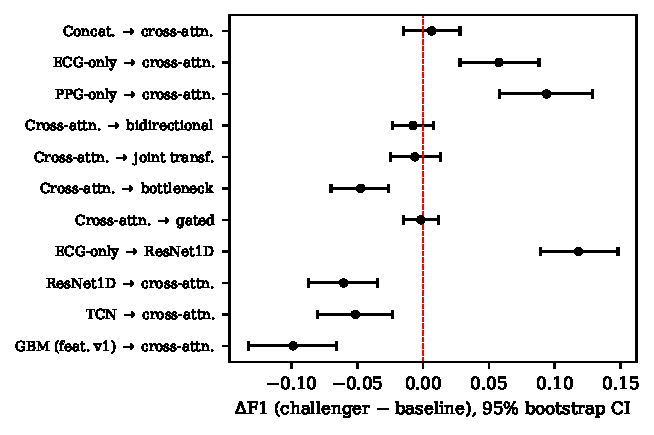
\includegraphics[width=\columnwidth]{figures/forest.pdf}
\caption{Paired F1 differences with 95\% bootstrap confidence intervals (Challenge 2015).}
\label{fig:forest}
\end{figure}

The four attention-style fusion variants cannot be told apart from each other or from concatenation. The bootstrap supports a benefit of fusion over either single signal, but the more conservative Nadeau-Bengio test does not after Holm correction. By our own rule (both tests must agree), only comparisons such as GBM versus cross-attention count as robust. The disagreement is expected, because the corrected $t$-test accounts for overlapping training sets.

\subsection{Per-alarm-type behavior}
Table~\ref{tab:type} shows pooled out-of-fold results for cross-attention. Performance is highly type-dependent: tachycardia has an F1 of 0.92 but a specificity of only 0.42, VT has F1 0.49, and asystole and ventricular flutter/fibrillation have too few true alarms (14 and 5) for reliable conclusions. In the error taxonomy, persistent missed true alarms are dominated by VT (18 of 29 persistent false negatives for the feature GBM, although VT is only 26\% of true alarms).

\begin{table}[t]
\caption{Cross-attention per alarm type (Challenge 2015, pooled out-of-fold).}
\label{tab:type}
\centering
\small
\begin{tabular}{lrrccc}
\toprule
Alarm type & $n$ & True & F1 & Sens. & Spec.\\
\midrule
Asystole & 93 & 14 & 0.41 & 0.56 & 0.80\\
Bradycardia & 73 & 39 & 0.75 & 0.69 & 0.83\\
Tachycardia & 111 & 106 & 0.92 & 0.87 & 0.42\\
V. flutter/fib. & 45 & 5 & 0.26 & 0.42 & 0.77\\
V. tachycardia & 270 & 59 & 0.49 & 0.58 & 0.78\\
\bottomrule
\end{tabular}
\end{table}

\subsection{Do fusion models use ECG-to-pulse timing?}
The original design rests on this question. Perturbing one modality while the other is intact (seed-0 checkpoints, five test folds; Fig.~\ref{fig:cf}) shows that replacing the PPG by another patient's \emph{same-label} PPG, whose timing is unrelated to the ECG, changes AUC by only 0.00 to 0.03 (cross-attention 0.002, concatenation 0.015, ResNet1D 0.021, TCN 0.024). Shifting the PPG by up to 2~s changes AUC by at most 0.005 for the CNN fusion models and by 0.03 to 0.06 for ResNet1D, TCN, InceptionTime and BiGRU. In contrast, an \emph{opposite-label} pulse collapses AUC (cross-attention 0.842 to 0.535). The models use the \emph{content} of each signal (morphology, regularity, presence of a pulse) as evidence, not the beat-to-pulse timing.

\begin{figure}[t]
\centering
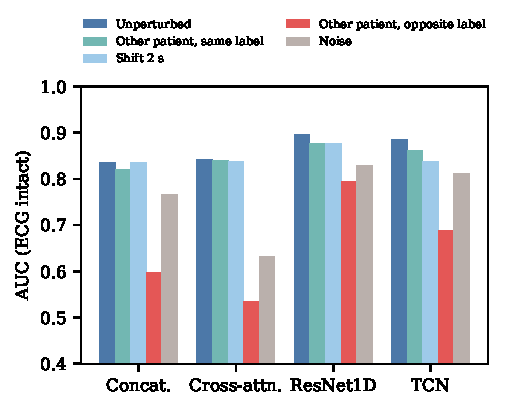
\includegraphics[width=\columnwidth]{figures/counterfactual.pdf}
\caption{Test AUC when the PPG is perturbed and the ECG is intact.}
\label{fig:cf}
\end{figure}

The attention maps agree. The attention-implied lag shows no relationship with the measured PTT (window-level Spearman $\rho=-0.039$, permutation $p=0.39$; beat-level $\rho=0.017$), and only 5.3\% of attention mass falls in the physiological lag range versus 5.6\% for uniform attention (Fig.~\ref{fig:ptt}). In deletion/insertion tests, occlusion is clearly faithful (PPG deletion $-0.041$, insertion $+0.041$) and integrated gradients modestly so ($-0.016$/$+0.010$), whereas attention weights are barely better than random ordering ($-0.007$/$+0.011$). Attention weights should not be presented as an explanation, and these data do not support the pulse-transit-time justification in our original proposal.

\begin{figure}[t]
\centering
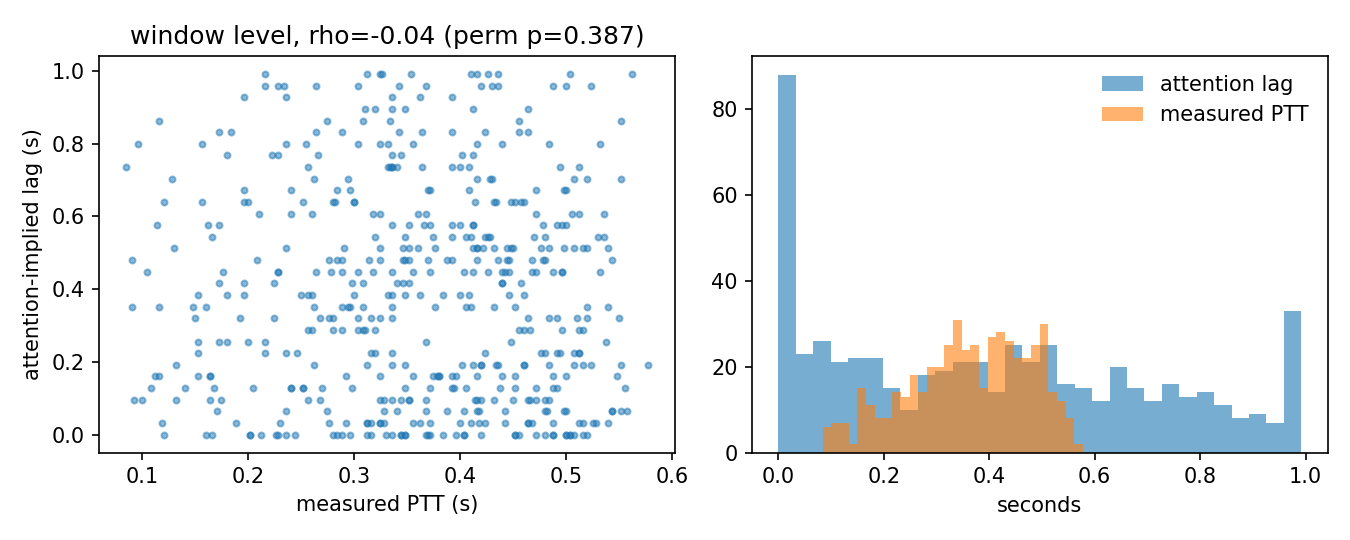
\includegraphics[width=\columnwidth]{figures/attention_vs_ptt.png}
\caption{Attention-implied lag versus measured PTT (left, window level) and the two lag distributions (right).}
\label{fig:ptt}
\end{figure}

\subsection{Robustness to noise and sensor loss}
With real Noise Stress Test noise on the ECG and synthetic motion artifact on the PPG (SNR 24 to 0~dB), ResNet1D is the most robust (AUC 0.907 clean to 0.844 at 0~dB on both signals), whereas cross-attention falls from 0.856 to 0.696 and concatenation from 0.833 to 0.720 (Fig.~\ref{fig:noise}). Zeroing the PPG at inference, without retraining, costs cross-attention 0.12 AUC (0.856 to 0.736), concatenation 0.10 and ResNet1D 0.27; zeroing the ECG costs cross-attention 0.08. Constant PPG delays of 0 to 400~ms barely change the CNN fusion models, consistent with the previous subsection. A check that the injected noise is not a learnable shortcut gave an AUC of 0.52 to 0.55 from model probabilities alone.

\begin{figure}[t]
\centering
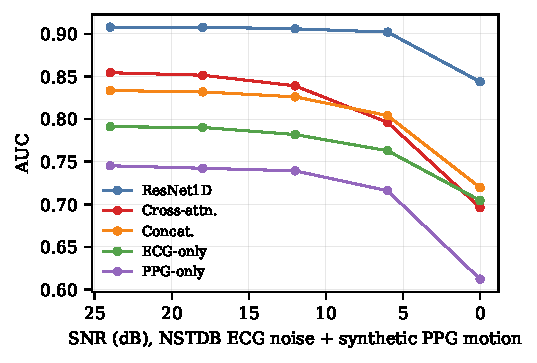
\includegraphics[width=\columnwidth]{figures/noise.pdf}
\caption{AUC versus injected noise level (mean over noise types; seed-0 checkpoints).}
\label{fig:noise}
\end{figure}

\subsection{Generalization across datasets}
Transfer is strongly asymmetric (Fig.~\ref{fig:transfer}). Models trained on the small Challenge 2015 set and tested on the VTaC test split reach F1 of 0.56 to 0.60 (AUC 0.73 to 0.78) when the ECG is used, whereas the PPG-only model is near chance (F1 0.432, AUC 0.541); in-distribution VTaC F1 is 0.71 to 0.78. In the other direction, models trained on VTaC transfer well to Challenge 2015 VT alarms (ResNet1D F1 0.773, AUC 0.927). For comparison, cross-attention trained and tested within Challenge 2015 reaches a VT F1 of only 0.49, so the amount of training data matters more than the model family, and single-dataset numbers overstate real-world performance.

\begin{figure}[t]
\centering
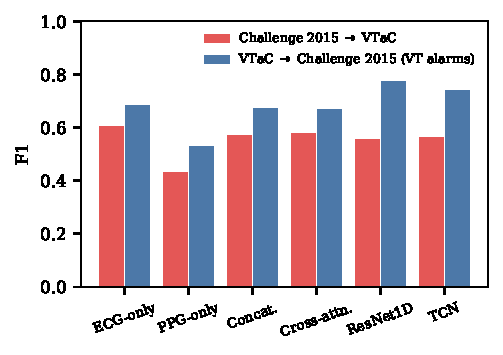
\includegraphics[width=\columnwidth]{figures/transfer.pdf}
\caption{Cross-dataset transfer (F1).}
\label{fig:transfer}
\end{figure}

\subsection{Pretraining, foundation models and AF screening}
Fine-tuning from self-supervised encoders gives modest paired gains over scratch training (+0.01 to +0.04 F1, three seeds, label fractions 10 to 100\%), but only 1 of 72 paired contrasts has a Nadeau-Bengio $p<0.05$, so the effect is suggestive rather than established. The PaPaGei foundation model did not beat from-scratch encoders: a frozen linear probe reached F1 0.58 (PPG alone) on Challenge 2015, and the best PaPaGei fusion model was about 0.04 F1 below scratch cross-attention; on VTaC it improved on a scratch PPG-only model (F1 0.58 to 0.62 versus 0.566) but not on scratch fusion (0.745). On the MIMIC PERform AF task (35 subjects, subject-wise cross-validation, low power) a gradient-boosting model on RR-irregularity features reached subject-level AUC 1.00 and was significantly better than the best neural model (0.93), while fusion beat a PPG-only network by $+0.28$ subject AUC. Distilling a PPG-only student from the fusion teacher gave no benefit over hard labels.

\subsection{Label reliability, time-to-verdict and safety}
On VTaC, 7.7\% of events (351 of 4,542) have split annotator votes, and accuracy is much lower on them (cross-attention 0.704 versus 0.854 on unanimous events); model entropy tracks disagreement only weakly (Spearman 0.13 to 0.18). Training on annotator vote fractions improved cross-attention by $+0.038$ F1 (SD 0.012, 5 seeds). A time-to-verdict analysis slides the 10~s window past the trigger and shows F1 falling (cross-attention 0.740, 0.713, 0.515 and 0.451 at 0, 5, 10 and 30~s); because the triggering event leaves the window, this is not evidence about whether waiting helps, and a design that appends post-alarm seconds to the pre-alarm window was not run.

A safety layer (temperature scaling, a risk-controlled threshold with a Clopper-Pearson bound, and a deferral band) was run for the concatenation model only. A 10\% miss tolerance at 90\% confidence could be certified in 42 of 50 folds, suppressing 22.5\% of false alarms while missing 2.9\% of true alarms, and calibration reduced the expected calibration error from 0.167 to 0.121. Thresholds aimed at 95 to 100\% validation sensitivity realized only about 92 to 97\% on test folds, so sensitivity targets must not be assumed to transfer.

\subsection{Limitations}
(i) The data are small: fold-to-fold F1 standard deviation is about 0.05, so many differences between top models are inside noise, and the standard deviations reported over seeds$\times$folds are not confidence intervals. (ii) Several engineered features, and on Challenge 2015 the alarm type itself, encode the alarm definitions; this is not learned physiology, and an ablation without the alarm type was not run. (iii) The hybrid recipe carries a small selection-bias risk. (iv) The Mousavi-style and contrastive reproductions are re-implementations from the published descriptions; only a two-seed sanity run of the former exists, so we make no claim about the original methods' performance. (v) There is no prospective validation, all data are from US ICUs, effects of demographics and skin tone on optical PPG were not assessed, VTaC device identifiers are not released (the lead-set signature used as a proxy is unverified), and patient overlap between corpora cannot be checked. (vi) Leave-one-device-out evaluation, long pre-alarm context, ECG-FM and pretraining on larger corpora (PulseDB, VitalDB, MIMIC-III) were not run because of time or data access. (vii) The model must not be used to suppress alarms unsupervised; the data are public and de-identified under the sources' IRB approvals.

%=====================================================================
\section{Conclusion}\label{sec:conclusion}
We tested whether cross-attention fusion of ECG and pulse signals verifies ICU arrhythmia alarms better than simpler alternatives. Under a leakage-free protocol it does not. The originally proposed model is no better than naive concatenation, and engineered-feature classifiers, a carefully trained hybrid attention CNN-GRU and ensembles clearly beat it (accuracy 0.878 to 0.913, F1 0.83 to 0.86). The two signals do complement each other, since fusion beats either signal alone on VTaC. But the models use the content of each signal, not the beat-to-pulse timing that motivated the design; the counterfactual tests and the attention-PTT analysis agree on this. An unnoticed validation leak had inflated our headline F1 by 0.075, and the controlled protocol is what makes the remaining conclusions trustworthy. Next steps are leave-one-site-out evaluation, larger unlabeled pretraining corpora and prospective validation. Code, configurations and result files are in the project repository.

\section*{Acknowledgment}
The authors thank the PhysioNet teams and the dataset creators cited in Table~\ref{tab:datasets}. [Add funding and supervisor acknowledgments.]

\bibliographystyle{IEEEtran}
\bibliography{references}

\end{document}
